\documentclass[hyperref={pdftex,unicode}]{beamer}

\usepackage[T2A]{fontenc}
\usepackage[utf8]{inputenc}
\usepackage[russian]{babel}
\usepackage{cmap}

\usepackage{xcolor}

\usepackage{helvet}
\usepackage{pscyr}

\usepackage{multicol}

\usepackage{amssymb,amsfonts,amsmath,mathtext}
\usepackage{cite,enumerate,float}

\usepackage{listings}
\usepackage{tikz}

\graphicspath{{images/}}
../../../templates/presentation/sys/styles.tex

\title{Численный анализ методов линейной аппроксимации статистических данных}
\author{%
    \small{Будный Р. И.} \\
    \smallskip
    \scriptsize{Научный руководитель: Муха В. С.}
}

\institute{
    Белорусский государственный университет информатики и радиоэлектроники
}
\date{2017}


\begin{document}

\begin{frame}
  \maketitle
\end{frame}

\begin{frame}{Постановка задачи}
  \centering% Graphic for TeX using PGF
% Title: /home/budnyjj/univer/magistracy/conferences/53/presentation/images/scheme.dia
% Creator: Dia v0.97.3
% CreationDate: Tue May  2 12:37:41 2017
% For: budnyjj
% \usepackage{tikz}
% The following commands are not supported in PSTricks at present
% We define them conditionally, so when they are implemented,
% this pgf file will use them.
\ifx\du\undefined
  \newlength{\du}
\fi
\setlength{\du}{15\unitlength}
\begin{tikzpicture}
\pgftransformxscale{1.000000}
\pgftransformyscale{-1.000000}
\definecolor{dialinecolor}{rgb}{0.000000, 0.000000, 0.000000}
\pgfsetstrokecolor{dialinecolor}
\definecolor{dialinecolor}{rgb}{1.000000, 1.000000, 1.000000}
\pgfsetfillcolor{dialinecolor}
\definecolor{dialinecolor}{rgb}{1.000000, 1.000000, 1.000000}
\pgfsetfillcolor{dialinecolor}
\fill (14.000000\du,14.000000\du)--(14.000000\du,15.900000\du)--(18.145000\du,15.900000\du)--(18.145000\du,14.000000\du)--cycle;
\pgfsetlinewidth{0.100000\du}
\pgfsetdash{}{0pt}
\pgfsetdash{}{0pt}
\pgfsetmiterjoin
\definecolor{dialinecolor}{rgb}{0.000000, 0.000000, 0.000000}
\pgfsetstrokecolor{dialinecolor}
\draw (14.000000\du,14.000000\du)--(14.000000\du,15.900000\du)--(18.145000\du,15.900000\du)--(18.145000\du,14.000000\du)--cycle;
% setfont left to latex
\definecolor{dialinecolor}{rgb}{0.000000, 0.000000, 0.000000}
\pgfsetstrokecolor{dialinecolor}
\node at (16.072500\du,15.000000\du){О: $ \alpha + \beta \xi $};
\definecolor{dialinecolor}{rgb}{1.000000, 1.000000, 1.000000}
\pgfsetfillcolor{dialinecolor}
\fill (9.000000\du,18.000000\du)--(9.000000\du,19.900000\du)--(13.122500\du,19.900000\du)--(13.122500\du,18.000000\du)--cycle;
\pgfsetlinewidth{0.100000\du}
\pgfsetdash{}{0pt}
\pgfsetdash{}{0pt}
\pgfsetmiterjoin
\definecolor{dialinecolor}{rgb}{0.000000, 0.000000, 0.000000}
\pgfsetstrokecolor{dialinecolor}
\draw (9.000000\du,18.000000\du)--(9.000000\du,19.900000\du)--(13.122500\du,19.900000\du)--(13.122500\du,18.000000\du)--cycle;
% setfont left to latex
\definecolor{dialinecolor}{rgb}{0.000000, 0.000000, 0.000000}
\pgfsetstrokecolor{dialinecolor}
\node at (11.061250\du,19.000000\du){И$_1$: $ \xi + \varepsilon $};
\definecolor{dialinecolor}{rgb}{1.000000, 1.000000, 1.000000}
\pgfsetfillcolor{dialinecolor}
\fill (19.000000\du,18.000000\du)--(19.000000\du,19.900000\du)--(23.135000\du,19.900000\du)--(23.135000\du,18.000000\du)--cycle;
\pgfsetlinewidth{0.100000\du}
\pgfsetdash{}{0pt}
\pgfsetdash{}{0pt}
\pgfsetmiterjoin
\definecolor{dialinecolor}{rgb}{0.000000, 0.000000, 0.000000}
\pgfsetstrokecolor{dialinecolor}
\draw (19.000000\du,18.000000\du)--(19.000000\du,19.900000\du)--(23.135000\du,19.900000\du)--(23.135000\du,18.000000\du)--cycle;
% setfont left to latex
\definecolor{dialinecolor}{rgb}{0.000000, 0.000000, 0.000000}
\pgfsetstrokecolor{dialinecolor}
\node at (21.067500\du,19.000000\du){И$_2$: $ \eta + \delta $};
\definecolor{dialinecolor}{rgb}{1.000000, 1.000000, 1.000000}
\pgfsetfillcolor{dialinecolor}
\fill (15.000000\du,18.000000\du)--(15.000000\du,19.900000\du)--(17.000000\du,19.900000\du)--(17.000000\du,18.000000\du)--cycle;
\pgfsetlinewidth{0.100000\du}
\pgfsetdash{}{0pt}
\pgfsetdash{}{0pt}
\pgfsetmiterjoin
\definecolor{dialinecolor}{rgb}{0.000000, 0.000000, 0.000000}
\pgfsetstrokecolor{dialinecolor}
\draw (15.000000\du,18.000000\du)--(15.000000\du,19.900000\du)--(17.000000\du,19.900000\du)--(17.000000\du,18.000000\du)--cycle;
% setfont left to latex
\definecolor{dialinecolor}{rgb}{0.000000, 0.000000, 0.000000}
\pgfsetstrokecolor{dialinecolor}
\node at (16.000000\du,19.000000\du){ВУ};
% setfont left to latex
\definecolor{dialinecolor}{rgb}{0.000000, 0.000000, 0.000000}
\pgfsetstrokecolor{dialinecolor}
\node[anchor=west] at (16.072500\du,14.950000\du){};
\pgfsetlinewidth{0.100000\du}
\pgfsetdash{}{0pt}
\pgfsetdash{}{0pt}
\pgfsetbuttcap
{
\definecolor{dialinecolor}{rgb}{0.000000, 0.000000, 0.000000}
\pgfsetfillcolor{dialinecolor}
% was here!!!
\pgfsetarrowsend{stealth}
\definecolor{dialinecolor}{rgb}{0.000000, 0.000000, 0.000000}
\pgfsetstrokecolor{dialinecolor}
\draw (8.000000\du,15.000000\du)--(13.950907\du,14.963141\du);
}
% setfont left to latex
\definecolor{dialinecolor}{rgb}{0.000000, 0.000000, 0.000000}
\pgfsetstrokecolor{dialinecolor}
\node[anchor=west] at (7.700000\du,14.300000\du){$ \xi $};
% setfont left to latex
\definecolor{dialinecolor}{rgb}{0.000000, 0.000000, 0.000000}
\pgfsetstrokecolor{dialinecolor}
\node[anchor=west] at (16.072500\du,14.950000\du){};
% setfont left to latex
\definecolor{dialinecolor}{rgb}{0.000000, 0.000000, 0.000000}
\pgfsetstrokecolor{dialinecolor}
\node[anchor=west] at (7.500000\du,14.000000\du){};
\pgfsetlinewidth{0.100000\du}
\pgfsetdash{}{0pt}
\pgfsetdash{}{0pt}
\pgfsetbuttcap
{
\definecolor{dialinecolor}{rgb}{0.000000, 0.000000, 0.000000}
\pgfsetfillcolor{dialinecolor}
% was here!!!
\pgfsetarrowsend{stealth}
\definecolor{dialinecolor}{rgb}{0.000000, 0.000000, 0.000000}
\pgfsetstrokecolor{dialinecolor}
\draw (18.145000\du,14.950000\du)--(24.000000\du,15.000000\du);
}
% setfont left to latex
\definecolor{dialinecolor}{rgb}{0.000000, 0.000000, 0.000000}
\pgfsetstrokecolor{dialinecolor}
\node[anchor=west] at (23.300000\du,14.300000\du){$ \eta $};
% setfont left to latex
\definecolor{dialinecolor}{rgb}{0.000000, 0.000000, 0.000000}
\pgfsetstrokecolor{dialinecolor}
\node[anchor=west] at (25.500000\du,14.500000\du){};
\pgfsetlinewidth{0.100000\du}
\pgfsetdash{}{0pt}
\pgfsetdash{}{0pt}
\pgfsetbuttcap
{
\definecolor{dialinecolor}{rgb}{0.000000, 0.000000, 0.000000}
\pgfsetfillcolor{dialinecolor}
% was here!!!
\pgfsetarrowsend{stealth}
\definecolor{dialinecolor}{rgb}{0.000000, 0.000000, 0.000000}
\pgfsetstrokecolor{dialinecolor}
\draw (10.975453\du,14.981570\du)--(11.039623\du,17.949657\du);
}
\pgfsetlinewidth{0.100000\du}
\pgfsetdash{}{0pt}
\pgfsetdash{}{0pt}
\pgfsetbuttcap
{
\definecolor{dialinecolor}{rgb}{0.000000, 0.000000, 0.000000}
\pgfsetfillcolor{dialinecolor}
% was here!!!
\pgfsetarrowsend{stealth}
\definecolor{dialinecolor}{rgb}{0.000000, 0.000000, 0.000000}
\pgfsetstrokecolor{dialinecolor}
\draw (21.072500\du,14.975000\du)--(21.068758\du,17.949942\du);
}
% setfont left to latex
\definecolor{dialinecolor}{rgb}{0.000000, 0.000000, 0.000000}
\pgfsetstrokecolor{dialinecolor}
\node[anchor=west] at (11.061250\du,18.950000\du){};
% setfont left to latex
\definecolor{dialinecolor}{rgb}{0.000000, 0.000000, 0.000000}
\pgfsetstrokecolor{dialinecolor}
\node[anchor=west] at (21.067500\du,18.950000\du){};
\pgfsetlinewidth{0.100000\du}
\pgfsetdash{}{0pt}
\pgfsetdash{}{0pt}
\pgfsetbuttcap
{
\definecolor{dialinecolor}{rgb}{0.000000, 0.000000, 0.000000}
\pgfsetfillcolor{dialinecolor}
% was here!!!
\pgfsetarrowsend{stealth}
\definecolor{dialinecolor}{rgb}{0.000000, 0.000000, 0.000000}
\pgfsetstrokecolor{dialinecolor}
\draw (19.000000\du,18.950000\du)--(17.049561\du,18.950000\du);
}
\pgfsetlinewidth{0.100000\du}
\pgfsetdash{}{0pt}
\pgfsetdash{}{0pt}
\pgfsetbuttcap
{
\definecolor{dialinecolor}{rgb}{0.000000, 0.000000, 0.000000}
\pgfsetfillcolor{dialinecolor}
% was here!!!
\pgfsetarrowsend{stealth}
\definecolor{dialinecolor}{rgb}{0.000000, 0.000000, 0.000000}
\pgfsetstrokecolor{dialinecolor}
\draw (13.122500\du,18.950000\du)--(15.000000\du,18.950000\du);
}
% setfont left to latex
\definecolor{dialinecolor}{rgb}{0.000000, 0.000000, 0.000000}
\pgfsetstrokecolor{dialinecolor}
\node[anchor=west] at (13.550000\du,18.400000\du){$ x $};
% setfont left to latex
\definecolor{dialinecolor}{rgb}{0.000000, 0.000000, 0.000000}
\pgfsetstrokecolor{dialinecolor}
\node[anchor=west] at (17.550000\du,18.400000\du){$ y $};
% setfont left to latex
\definecolor{dialinecolor}{rgb}{0.000000, 0.000000, 0.000000}
\pgfsetstrokecolor{dialinecolor}
\node[anchor=west] at (18.000000\du,17.000000\du){};
\pgfsetlinewidth{0.100000\du}
\pgfsetdash{}{0pt}
\pgfsetdash{}{0pt}
\pgfsetbuttcap
{
\definecolor{dialinecolor}{rgb}{0.000000, 0.000000, 0.000000}
\pgfsetfillcolor{dialinecolor}
% was here!!!
\pgfsetarrowsend{stealth}
\definecolor{dialinecolor}{rgb}{0.000000, 0.000000, 0.000000}
\pgfsetstrokecolor{dialinecolor}
\draw (16.000000\du,19.900000\du)--(16.000000\du,21.000000\du);
}
% setfont left to latex
\definecolor{dialinecolor}{rgb}{0.000000, 0.000000, 0.000000}
\pgfsetstrokecolor{dialinecolor}
\node[anchor=west] at (15.100000\du,21.700000\du){$ \hat{\alpha}, \hat{\beta} $};
% setfont left to latex
\definecolor{dialinecolor}{rgb}{0.000000, 0.000000, 0.000000}
\pgfsetstrokecolor{dialinecolor}
\node[anchor=west] at (16.072500\du,14.950000\du){};
% setfont left to latex
\definecolor{dialinecolor}{rgb}{0.000000, 0.000000, 0.000000}
\pgfsetstrokecolor{dialinecolor}
\node[anchor=west] at (11.061250\du,18.950000\du){};
% setfont left to latex
\definecolor{dialinecolor}{rgb}{0.000000, 0.000000, 0.000000}
\pgfsetstrokecolor{dialinecolor}
\node[anchor=west] at (21.067500\du,18.950000\du){};
% setfont left to latex
\definecolor{dialinecolor}{rgb}{0.000000, 0.000000, 0.000000}
\pgfsetstrokecolor{dialinecolor}
\node[anchor=west] at (20.000000\du,22.000000\du){};
% setfont left to latex
\definecolor{dialinecolor}{rgb}{0.000000, 0.000000, 0.000000}
\pgfsetstrokecolor{dialinecolor}
\node[anchor=west] at (14.000000\du,18.500000\du){};
% setfont left to latex
\definecolor{dialinecolor}{rgb}{0.000000, 0.000000, 0.000000}
\pgfsetstrokecolor{dialinecolor}
\node[anchor=west] at (18.000000\du,17.000000\du){};
\end{tikzpicture}


  \flushleft{
    $ \xi, \eta $ --- фактические значения входа и выхода, \\
    $ \alpha, \beta $ --- параметры объекта, \\
    $ \varepsilon, \delta $ --- ошибки измерений, \\
    $ x, y $ --- измеряемые значения входа и выхода, \\
    $ \hat{\alpha}, \hat{\beta} $ --- оценки параметров объекта.
  }
\end{frame}

\begin{frame}{Постановка задачи}
  \begin{minipage}[h]{0.45\linewidth}
    \centering классическая \\ аппроксимация

    % Graphic for TeX using PGF
% Title: /home/budnyjj/univer/magistracy/conferences/53/presentation/images/classic.dia
% Creator: Dia v0.97.3
% CreationDate: Tue May  2 14:01:26 2017
% For: budnyjj
% \usepackage{tikz}
% The following commands are not supported in PSTricks at present
% We define them conditionally, so when they are implemented,
% this pgf file will use them.
\ifx\du\undefined
  \newlength{\du}
\fi
\setlength{\du}{15\unitlength}
\begin{tikzpicture}
\pgftransformxscale{0.700000}
\pgftransformyscale{-0.700000}
\definecolor{dialinecolor}{rgb}{0.000000, 0.000000, 0.000000}
\pgfsetstrokecolor{dialinecolor}
\definecolor{dialinecolor}{rgb}{1.000000, 1.000000, 1.000000}
\pgfsetfillcolor{dialinecolor}
\pgfsetlinewidth{0.100000\du}
\pgfsetdash{}{0pt}
\pgfsetdash{}{0pt}
\pgfsetbuttcap
{
\definecolor{dialinecolor}{rgb}{0.000000, 0.000000, 0.000000}
\pgfsetfillcolor{dialinecolor}
% was here!!!
\pgfsetarrowsend{stealth}
\definecolor{dialinecolor}{rgb}{0.000000, 0.000000, 0.000000}
\pgfsetstrokecolor{dialinecolor}
\draw (15.950000\du,22.050000\du)--(16.000000\du,13.000000\du);
}
\pgfsetlinewidth{0.100000\du}
\pgfsetdash{}{0pt}
\pgfsetdash{}{0pt}
\pgfsetbuttcap
{
\definecolor{dialinecolor}{rgb}{0.000000, 0.000000, 0.000000}
\pgfsetfillcolor{dialinecolor}
% was here!!!
\pgfsetarrowsend{stealth}
\definecolor{dialinecolor}{rgb}{0.000000, 0.000000, 0.000000}
\pgfsetstrokecolor{dialinecolor}
\draw (15.000000\du,21.000000\du)--(28.000000\du,21.000000\du);
}
\pgfsetlinewidth{0.100000\du}
\pgfsetdash{}{0pt}
\pgfsetdash{}{0pt}
\pgfsetbuttcap
{
\definecolor{dialinecolor}{rgb}{0.000000, 0.000000, 0.000000}
\pgfsetfillcolor{dialinecolor}
% was here!!!
\definecolor{dialinecolor}{rgb}{0.000000, 0.000000, 0.000000}
\pgfsetstrokecolor{dialinecolor}
\draw (18.000000\du,14.000000\du)--(26.000000\du,20.000000\du);
}
\pgfsetlinewidth{0.100000\du}
\pgfsetdash{{1.000000\du}{1.000000\du}}{0\du}
\pgfsetdash{{0.600000\du}{0.600000\du}}{0\du}
\pgfsetbuttcap
{
\definecolor{dialinecolor}{rgb}{0.000000, 0.000000, 0.000000}
\pgfsetfillcolor{dialinecolor}
% was here!!!
}
\definecolor{dialinecolor}{rgb}{0.000000, 0.000000, 0.000000}
\pgfsetstrokecolor{dialinecolor}
\draw (20.000000\du,16.200000\du)--(20.000000\du,19.000000\du);
\pgfsetbuttcap
\pgfsetmiterjoin
\pgfsetdash{}{0pt}
\pgfsetlinewidth{0.100000\du}
\definecolor{dialinecolor}{rgb}{0.000000, 0.000000, 0.000000}
\pgfsetfillcolor{dialinecolor}
\pgfpathellipse{\pgfpoint{20.000000\du}{15.450000\du}}{\pgfpoint{0.250000\du}{0\du}}{\pgfpoint{0\du}{0.250000\du}}
\pgfusepath{fill}
\definecolor{dialinecolor}{rgb}{0.000000, 0.000000, 0.000000}
\pgfsetfillcolor{dialinecolor}
\fill (20.250000\du,16.200000\du)--(20.000000\du,15.700000\du)--(19.750000\du,16.200000\du)--cycle;
\pgfsetbuttcap
\pgfsetmiterjoin
\pgfsetdash{}{0pt}
\pgfsetlinewidth{0.100000\du}
\definecolor{dialinecolor}{rgb}{0.000000, 0.000000, 0.000000}
\pgfsetfillcolor{dialinecolor}
\pgfpathellipse{\pgfpoint{20.000000\du}{19.750000\du}}{\pgfpoint{0.250000\du}{0\du}}{\pgfpoint{0\du}{0.250000\du}}
\pgfusepath{fill}
\definecolor{dialinecolor}{rgb}{0.000000, 0.000000, 0.000000}
\pgfsetfillcolor{dialinecolor}
\fill (19.750000\du,19.000000\du)--(20.000000\du,19.500000\du)--(20.250000\du,19.000000\du)--cycle;
% setfont left to latex
\definecolor{dialinecolor}{rgb}{0.000000, 0.000000, 0.000000}
\pgfsetstrokecolor{dialinecolor}
\node[anchor=west] at (18.000000\du,17.800000\du){$ \rho_{\text{к}_i} $};
% setfont left to latex
\definecolor{dialinecolor}{rgb}{0.000000, 0.000000, 0.000000}
\pgfsetstrokecolor{dialinecolor}
\node[anchor=west] at (20.300000\du,20.000000\du){$ (x_i, y_i) $};
% setfont left to latex
\definecolor{dialinecolor}{rgb}{0.000000, 0.000000, 0.000000}
\pgfsetstrokecolor{dialinecolor}
\node[anchor=west] at (18.500000\du,20.000000\du){};
% setfont left to latex
\definecolor{dialinecolor}{rgb}{0.000000, 0.000000, 0.000000}
\pgfsetstrokecolor{dialinecolor}
\node[anchor=west] at (20.300000\du,15.000000\du){$ (x_i, \hat{\alpha}_{\text{к}} + \hat{\beta}_{\text{к}} x_i ) $};
\end{tikzpicture}


    \( \rho_{\text{к}} = \sum \rho_{\text{к}_i} \rightarrow \min \)
  \end{minipage}
  \hfill
  \begin{minipage}[h]{0.45\linewidth}
    \centering симметричная \\ аппроксимация

    % Graphic for TeX using PGF
% Title: /home/budnyjj/univer/magistracy/conferences/53/presentation/images/symmetric.dia
% Creator: Dia v0.97.3
% CreationDate: Tue May  2 14:15:14 2017
% For: budnyjj
% \usepackage{tikz}
% The following commands are not supported in PSTricks at present
% We define them conditionally, so when they are implemented,
% this pgf file will use them.
\ifx\du\undefined
  \newlength{\du}
\fi
\setlength{\du}{15\unitlength}
\begin{tikzpicture}
\pgftransformxscale{0.700000}
\pgftransformyscale{-0.700000}
\definecolor{dialinecolor}{rgb}{0.000000, 0.000000, 0.000000}
\pgfsetstrokecolor{dialinecolor}
\definecolor{dialinecolor}{rgb}{1.000000, 1.000000, 1.000000}
\pgfsetfillcolor{dialinecolor}
\pgfsetlinewidth{0.100000\du}
\pgfsetdash{}{0pt}
\pgfsetdash{}{0pt}
\pgfsetbuttcap
{
\definecolor{dialinecolor}{rgb}{0.000000, 0.000000, 0.000000}
\pgfsetfillcolor{dialinecolor}
% was here!!!
\pgfsetarrowsend{stealth}
\definecolor{dialinecolor}{rgb}{0.000000, 0.000000, 0.000000}
\pgfsetstrokecolor{dialinecolor}
\draw (15.950000\du,22.050000\du)--(16.000000\du,13.000000\du);
}
\pgfsetlinewidth{0.100000\du}
\pgfsetdash{}{0pt}
\pgfsetdash{}{0pt}
\pgfsetbuttcap
{
\definecolor{dialinecolor}{rgb}{0.000000, 0.000000, 0.000000}
\pgfsetfillcolor{dialinecolor}
% was here!!!
\pgfsetarrowsend{stealth}
\definecolor{dialinecolor}{rgb}{0.000000, 0.000000, 0.000000}
\pgfsetstrokecolor{dialinecolor}
\draw (15.000000\du,21.000000\du)--(28.000000\du,21.000000\du);
}
\pgfsetlinewidth{0.100000\du}
\pgfsetdash{}{0pt}
\pgfsetdash{}{0pt}
\pgfsetbuttcap
{
\definecolor{dialinecolor}{rgb}{0.000000, 0.000000, 0.000000}
\pgfsetfillcolor{dialinecolor}
% was here!!!
\definecolor{dialinecolor}{rgb}{0.000000, 0.000000, 0.000000}
\pgfsetstrokecolor{dialinecolor}
\draw (17.006017\du,14.015552\du)--(26.000000\du,18.000000\du);
}
\pgfsetlinewidth{0.100000\du}
\pgfsetdash{{1.000000\du}{1.000000\du}}{0\du}
\pgfsetdash{{0.600000\du}{0.600000\du}}{0\du}
\pgfsetbuttcap
{
\definecolor{dialinecolor}{rgb}{0.000000, 0.000000, 0.000000}
\pgfsetfillcolor{dialinecolor}
% was here!!!
}
\definecolor{dialinecolor}{rgb}{0.000000, 0.000000, 0.000000}
\pgfsetstrokecolor{dialinecolor}
\draw (21.552786\du,16.894427\du)--(20.447214\du,19.105573\du);
\pgfsetbuttcap
\pgfsetmiterjoin
\pgfsetdash{}{0pt}
\pgfsetlinewidth{0.100000\du}
\definecolor{dialinecolor}{rgb}{0.000000, 0.000000, 0.000000}
\pgfsetfillcolor{dialinecolor}
\pgfpathellipse{\pgfpoint{21.888197\du}{16.223607\du}}{\pgfpoint{0.250000\du}{0\du}}{\pgfpoint{0\du}{0.250000\du}}
\pgfusepath{fill}
\pgfpathellipse{\pgfpoint{20.111803\du}{15.3923607\du}}{\pgfpoint{0.250000\du}{0\du}}{\pgfpoint{0\du}{0.250000\du}}
\pgfusepath{fill}
\definecolor{dialinecolor}{rgb}{0.000000, 0.000000, 0.000000}
\pgfsetfillcolor{dialinecolor}
\fill (21.776393\du,17.006231\du)--(21.776393\du,16.447214\du)--(21.329180\du,16.782624\du)--cycle;
\pgfsetbuttcap
\pgfsetmiterjoin
\pgfsetdash{}{0pt}
\pgfsetlinewidth{0.100000\du}
\definecolor{dialinecolor}{rgb}{0.000000, 0.000000, 0.000000}
\pgfsetfillcolor{dialinecolor}
\pgfpathellipse{\pgfpoint{20.111803\du}{19.776393\du}}{\pgfpoint{0.250000\du}{0\du}}{\pgfpoint{0\du}{0.250000\du}}
\pgfusepath{fill}
\definecolor{dialinecolor}{rgb}{0.000000, 0.000000, 0.000000}
\pgfsetfillcolor{dialinecolor}
\fill (20.223607\du,18.993769\du)--(20.223607\du,19.552786\du)--(20.670820\du,19.217376\du)--cycle;
% setfont left to latex
\definecolor{dialinecolor}{rgb}{0.000000, 0.000000, 0.000000}
\pgfsetstrokecolor{dialinecolor}
\node[anchor=west] at (18.500000\du,18.000000\du){$ \rho_{\text{с}_i} $};
% setfont left to latex
\definecolor{dialinecolor}{rgb}{0.000000, 0.000000, 0.000000}
\pgfsetstrokecolor{dialinecolor}
\node[anchor=west] at (20.300000\du,20.000000\du){$ (x_i, y_i) $};
% setfont left to latex
\definecolor{dialinecolor}{rgb}{0.000000, 0.000000, 0.000000}
\pgfsetstrokecolor{dialinecolor}
\node[anchor=west] at (18.500000\du,20.000000\du){};
% setfont left to latex
\definecolor{dialinecolor}{rgb}{0.000000, 0.000000, 0.000000}
\pgfsetstrokecolor{dialinecolor}
\node[anchor=west] at (20.300000\du,14.700000\du){$ (x_i, \psi(\hat{\theta_{\text{с}}}, x_i)) $};
\end{tikzpicture}

    % $ \varepsilon = N(0, \sigma_{\varepsilon}), \delta = N(0, \sigma_{\delta}) $
    % --- ошибки измерений, \\


    \bigskip
    \( \rho_{\text{с}} = \sum \rho_{\text{с}_i} \rightarrow \min \)
  \end{minipage}
\end{frame}

\begin{frame}{Постановка задачи}
  Выполнить сравнение точности:
  \begin{itemize}
  \item оценивания значений параметров объекта;
  \item прогнозирования измеряемых значений выхода по измеряемым значениям входа.
  \end{itemize}
\end{frame}

\begin{frame}{Моделирование}
  Значения \( \xi \) выбирались из \( U(0, 10) \). \\
  Оценивание параметров \( \alpha, \beta \) производилось по измерениям
  \begin{align*}
    x_i &= \xi_i + \varepsilon_i, \varepsilon_i \in N(0, \sigma_{\varepsilon}), \\
    y_i &= \eta_i + \delta_i, \delta_i \in N(0, \sigma_{\delta}), \\
    i &= \overline{1, n}, \: n = 100.
  \end{align*}
  Расчеты производились в узлах сетки значений \( \sigma_{\varepsilon}, \sigma_{\delta} \) в \\
  прямоугольнике  \( [0, 2] \times [0, 2] \) с шагом 0{,}1. \\
  В каждом узле сетки вычислялось \( k = 100 \) оценок.
\end{frame}

\begin{frame}{Точность оценивания параметров объекта}
  \begin{center}\large
    \( d = \dfrac{1}{k} \sum_{j=1}^k \sqrt{(\hat{\alpha}_j - \alpha)^2 + (\hat{\beta}_j - \beta)^2} \).

    \bigskip
    \( D = d_{\text{к}} - d_{\text{с}}:
    \begin{cases}
      < 0, & \text{если классическая аппр. точнее}, \\
      = 0, & \text{если методы равноточные}, \\
      > 0, & \text{если симметричная аппр. точнее}.
    \end{cases} \)

    \bigskip
    \( D(\sigma_{\varepsilon}, \sigma_{\delta}) \) --- ?
  \end{center}
\end{frame}

\begin{frame}{Точность оценивания параметров объекта}
  \begin{minipage}[h]{0.49\linewidth}\centering
    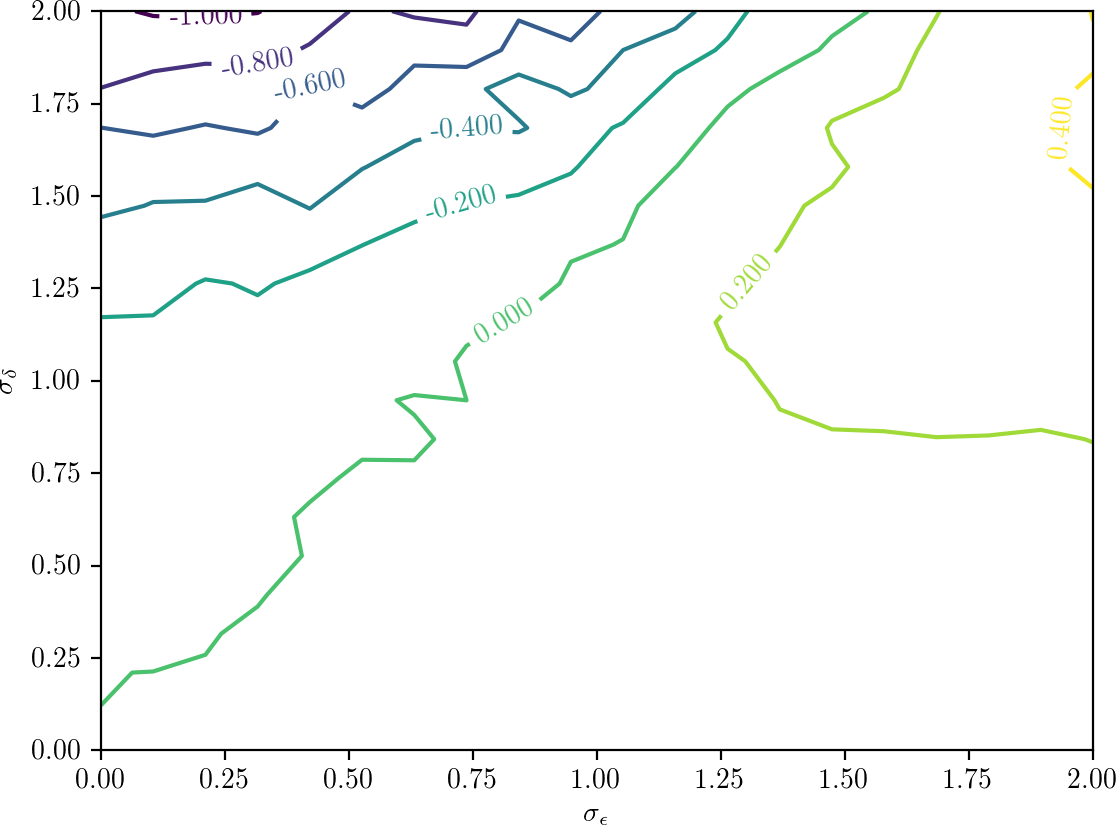
\includegraphics[width=\linewidth]{beta-0,5_param.png}

    \bigskip
    \scriptsize\( D(\sigma_{\varepsilon}, \sigma_{\delta}), \: \beta = 0{,}5 \)
  \end{minipage}
  \hfill
  \begin{minipage}[h]{0.49\linewidth}\centering
    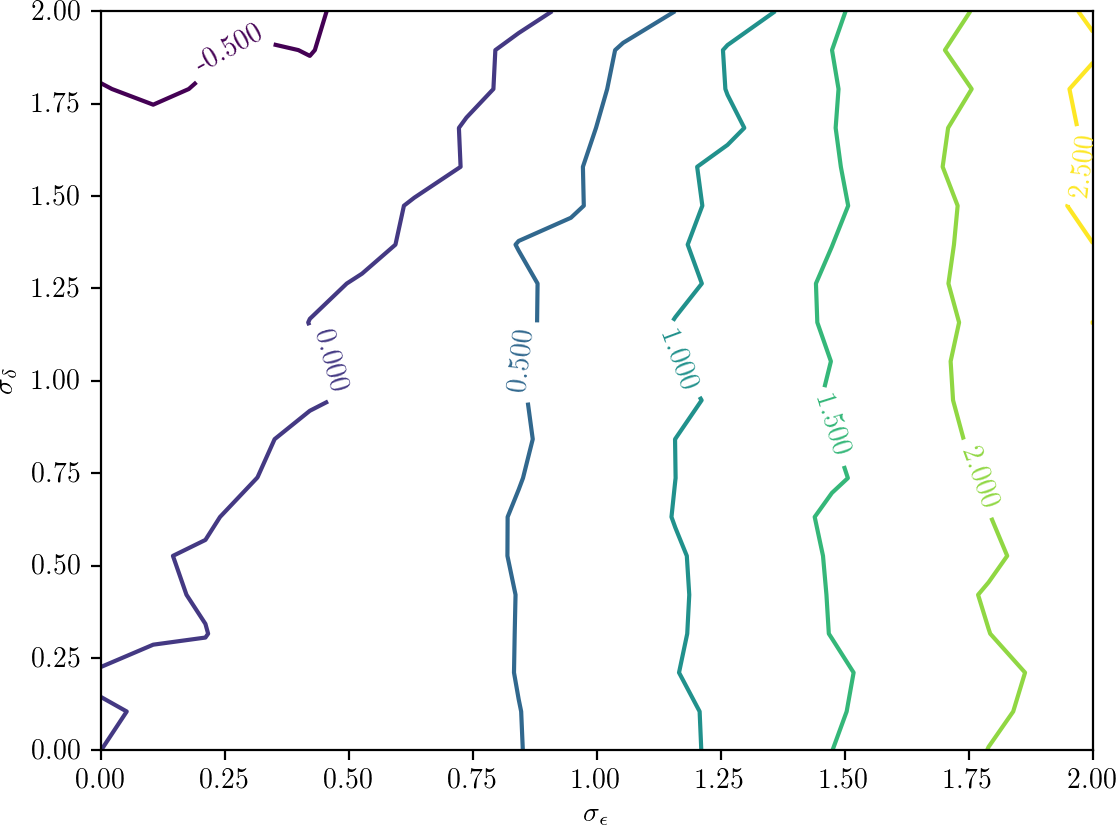
\includegraphics[width=\linewidth]{beta-2_param.png}

    \bigskip
    \scriptsize\( D(\sigma_{\varepsilon}, \sigma_{\delta}), \: \beta = 2 \)
  \end{minipage}
\end{frame}

\begin{frame}{Точность оценивания параметров объекта}
  \begin{minipage}[h]{0.49\linewidth}\centering
    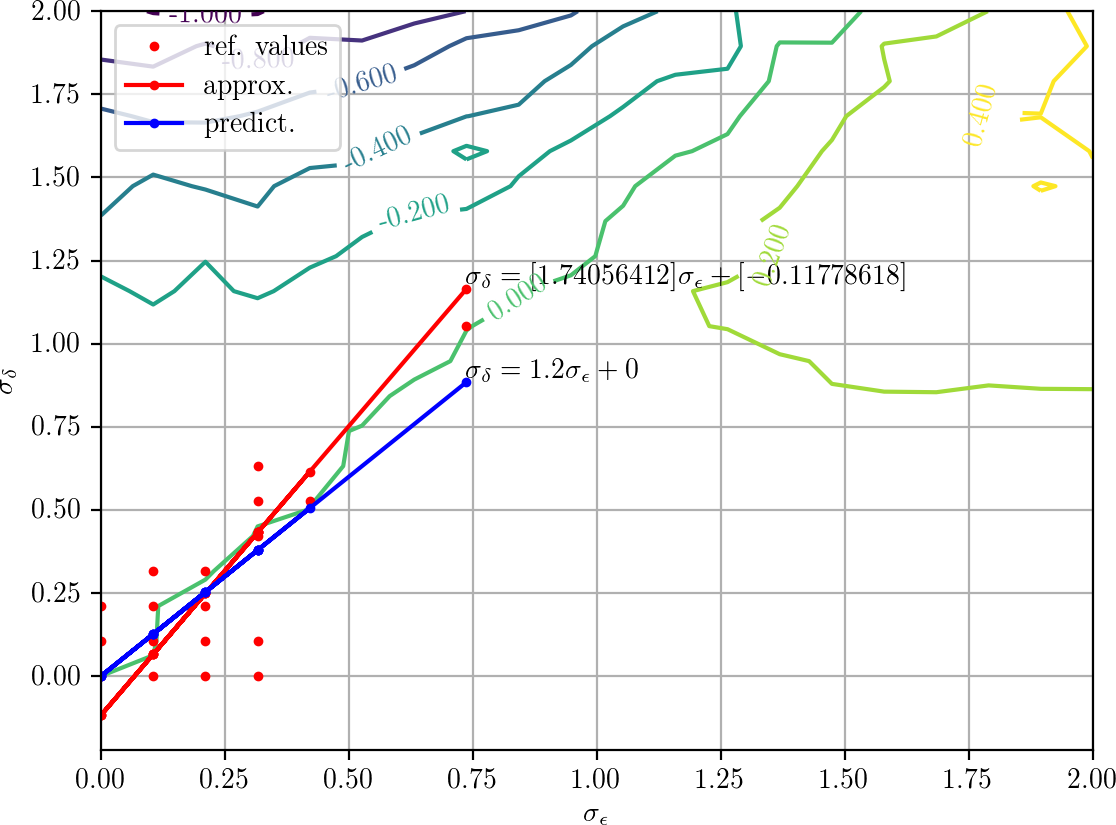
\includegraphics[width=\linewidth]{beta-0,5_param-accs-diff-approx.png}

    \bigskip
    \scriptsize\( D(\sigma_{\varepsilon}, \sigma_{\delta}), \: \beta = 0{,}5 \)
  \end{minipage}
  \hfill
  \begin{minipage}[h]{0.49\linewidth}\centering
    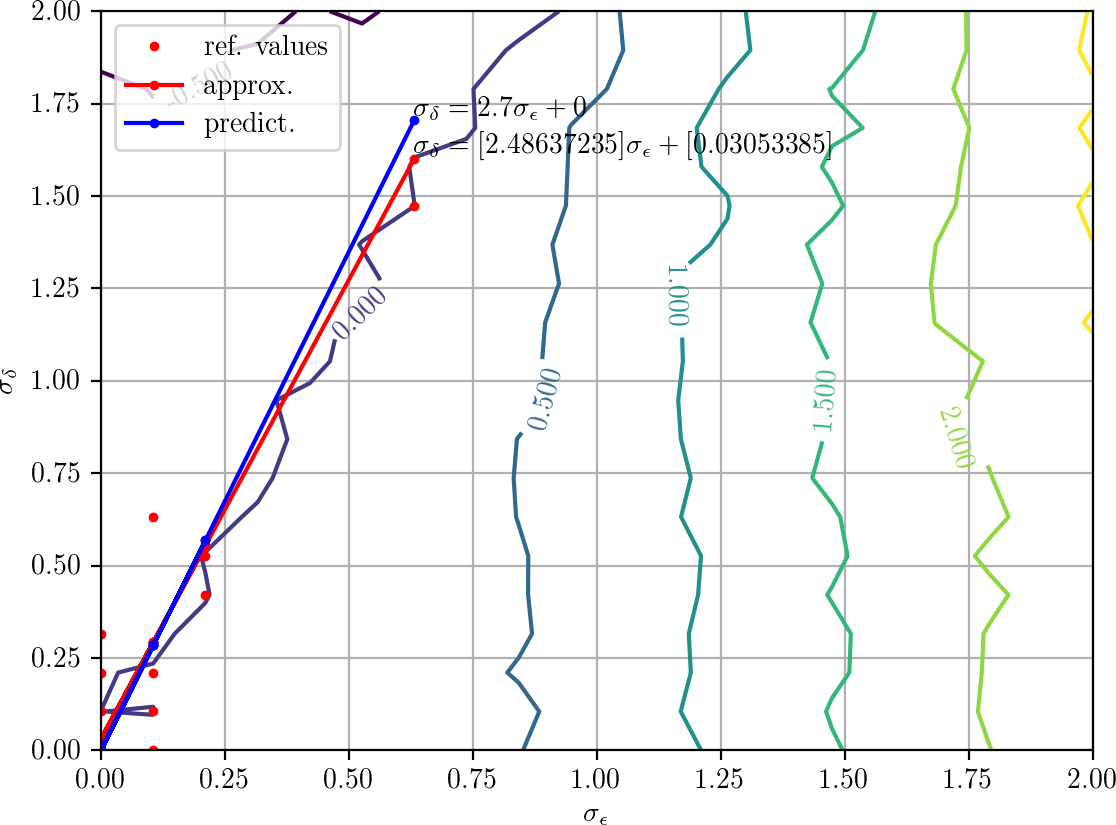
\includegraphics[width=\linewidth]{beta-2_param-accs-diff-approx.png}

    \bigskip
    \scriptsize\( D(\sigma_{\varepsilon}, \sigma_{\delta}), \: \beta = 2 \)
  \end{minipage}
\end{frame}

\begin{frame}{Точность оценивания параметров объекта}
  \begin{enumerate}
  \item Значения \( \alpha \) не влияют на точность оценивания.
  \item Если \( \sigma_{\delta} < (0,7 + |\beta|)\sigma_{\varepsilon} \),
    то оценки параметров, полученные методом симметричной аппроксимации,
    являются более точными, чем у классической \\
    линейной регрессии.
  \end{enumerate}
\end{frame}

\begin{frame}{Точность прогнозирования значений выхода}
  \begin{center}\large
    \( p = \dfrac{1}{k} \sum_{j=1}^k \sum_{i=1}^n |y_{ji} - (\hat{\alpha}_{j} + \hat{\beta}_{j} x_{ji})| \),

    \bigskip
    \( x_{ji}, y_{ji} \) --- контрольные измерения.

    \bigskip
    \( P = p_{\text{к}} - p_{\text{с}}:
    \begin{cases}
      < 0, & \text{если классическая аппр. точнее}, \\
      = 0, & \text{если методы равноточные}, \\
      > 0, & \text{если симметричная аппр. точнее}.
    \end{cases} \)

    \bigskip
    \( P(\sigma_{\varepsilon}, \sigma_{\delta}) \) --- ?
  \end{center}
\end{frame}

\begin{frame}{Точность прогнозирования значений выхода}
  \begin{minipage}[h]{0.49\linewidth}\centering
    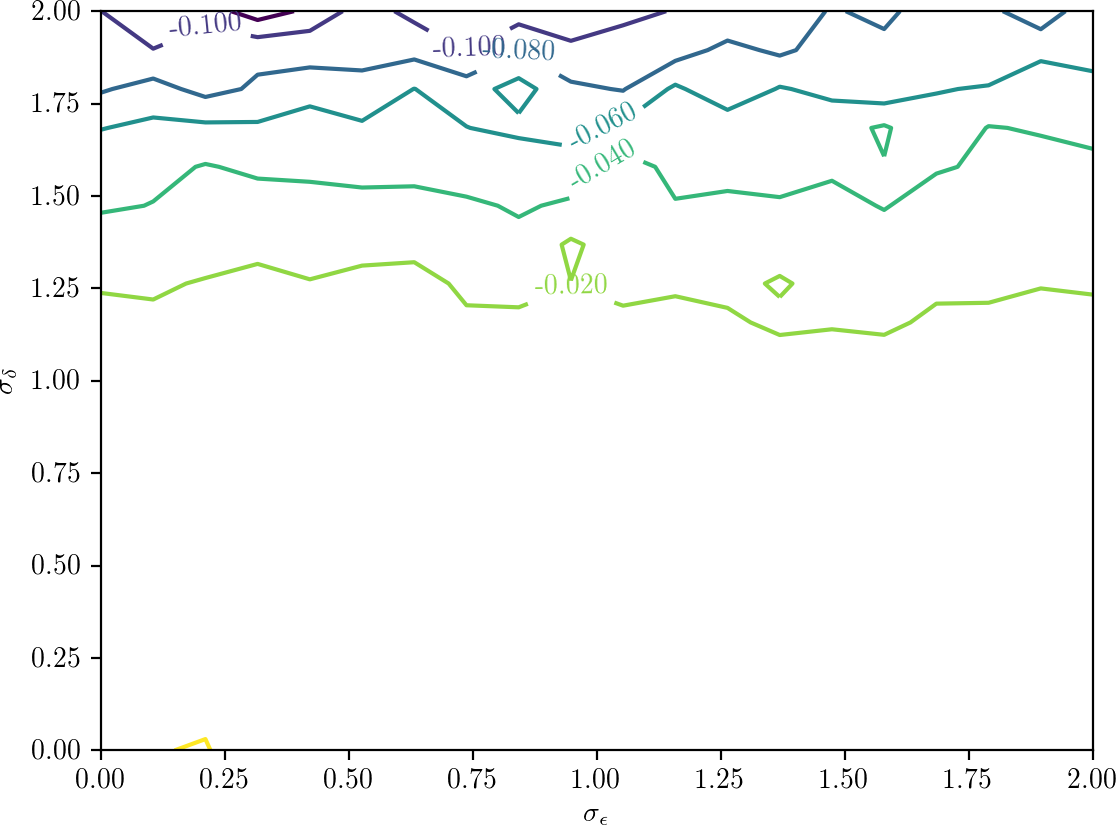
\includegraphics[width=\linewidth]{beta-0,5_predict-measured.png}

    \bigskip
    \scriptsize\( P(\sigma_{\varepsilon}, \sigma_{\delta}), \: \beta = 0{,}5 \)
  \end{minipage}
  \hfill
  \begin{minipage}[h]{0.49\linewidth}\centering
    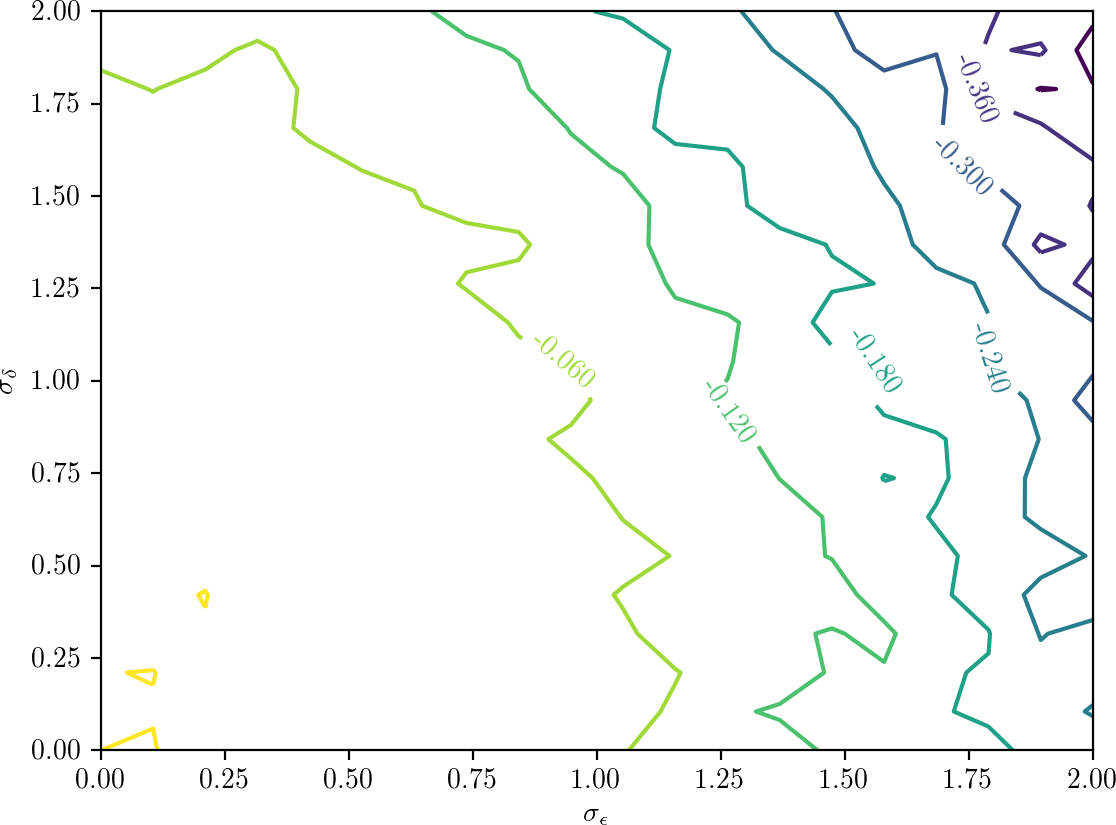
\includegraphics[width=\linewidth]{beta-2_predict-measured.png}

    \bigskip
    \scriptsize\( P(\sigma_{\varepsilon}, \sigma_{\delta}), \: \beta = 2 \)
  \end{minipage}
\end{frame}

\begin{frame}{Выводы}
  \begin{itemize}
  \item Точность оценивания параметров объекта рассматриваемыми
    методами зависит от значения \( \beta \). \\
    С ростом величины \( \beta \) оценки параметров,
    полученные методом симметричной аппроксимации, оказываются более точными.
    В противном случае, оценки, полученные классической аппроксимацией,
    имеют большую точность.
  \item Для определения того, какой из методов дает более точные оценки параметров,
    можно использовать следующее эмпирическое правило:
    \begin{center}
      \( \sigma_{\delta} < (0,7 + |\beta|)\sigma_{\varepsilon} \).
    \end{center}
  \item Классическая аппроксимация дает более точные прогнозы измеряемых
    значений выхода по измеряемым значениям входа для любых
    \( \beta, \sigma_{\varepsilon}, \sigma_{\delta} \).
  \end{itemize}
\end{frame}

\begin{frame}{Список литературы}
  \begin{enumerate}
  \item Рао, С. Р. Линейные статистические методы и их применение /
    С. Р. Рао. --- М.: Наука, 1968. --- 548 с.
  \item Pearson, K. On lines and planes of closest fit to systems of points in space /
    K. Pearson / Philosophical Magazine. --- 1901. --- V. VI. --- №2. --- P. 559 --- 572.
  \item Муха В. С.
    <<Симметричная аппроксимация векторных статистических данных линейными многообразиями>> //
    Весцi Нац. акад. навук Беларусi. Сер. фiз.-мат. навук. --- 2016. --- №4. --- С. 23--31.
  \end{enumerate}
\end{frame}

\end{document}